\subsection{Umsetzung des UI} %TODO UI Implementierung update nach Entwicklung
Die grafische Darstellung der ermittelten Messdaten wird in den folgenden Kapitel beschrieben.

\subsubsection{Webbrowser Client} 
Nach Aufgabenstellung wird ein web basierender Zugriff auf die ermittelten Messdaten gefordert. Dieser ist im Kontextdiagramm (Bild \ref{fig:kontext}) innerhalb der Systemgrenze als Web Client definiert.\\
Unter einem Web Client ist eine, auf dem Browser laufende Applikation zu verstehen.\\
\\
Der Zugriff auf die Messdaten läuft über die wohl definierte REST Schnittstelle, welche im Kapitel \ref{sec:rest} genauer erklärt ist. Dieser gekapselte Zugriff ermöglicht es eine unabhängige Darstellung zu implementieren.\\
Weiter gibt es die Möglichkeit andere grafische Benutzeroberflächen zu entwickeln, welche die gleichen Datengrundlagen haben.\\
\\
Der Aufbau des Clients erfolgt mittels eines Bootstrap Templates\footnote{Bootstrap Template von \cite{bootstrap}}. Im oberen Bereich wird die Temperatur, Feuchtigkeit, aktuelle Abweichung und Abweichung seit Beginn dargestellt. Darunter folgt ein Liniendiagramm, das den Ablauf der Abweichung pro Tag darstellt.Daneben ist eine Tagestabelle, die die Messergebnisse eines Tages anzeigt.\\
Das Liniendiagramm sowie die Tagestabelle können nach Datum gefiltert werden.

\begin{figure}[H]
    \centering
    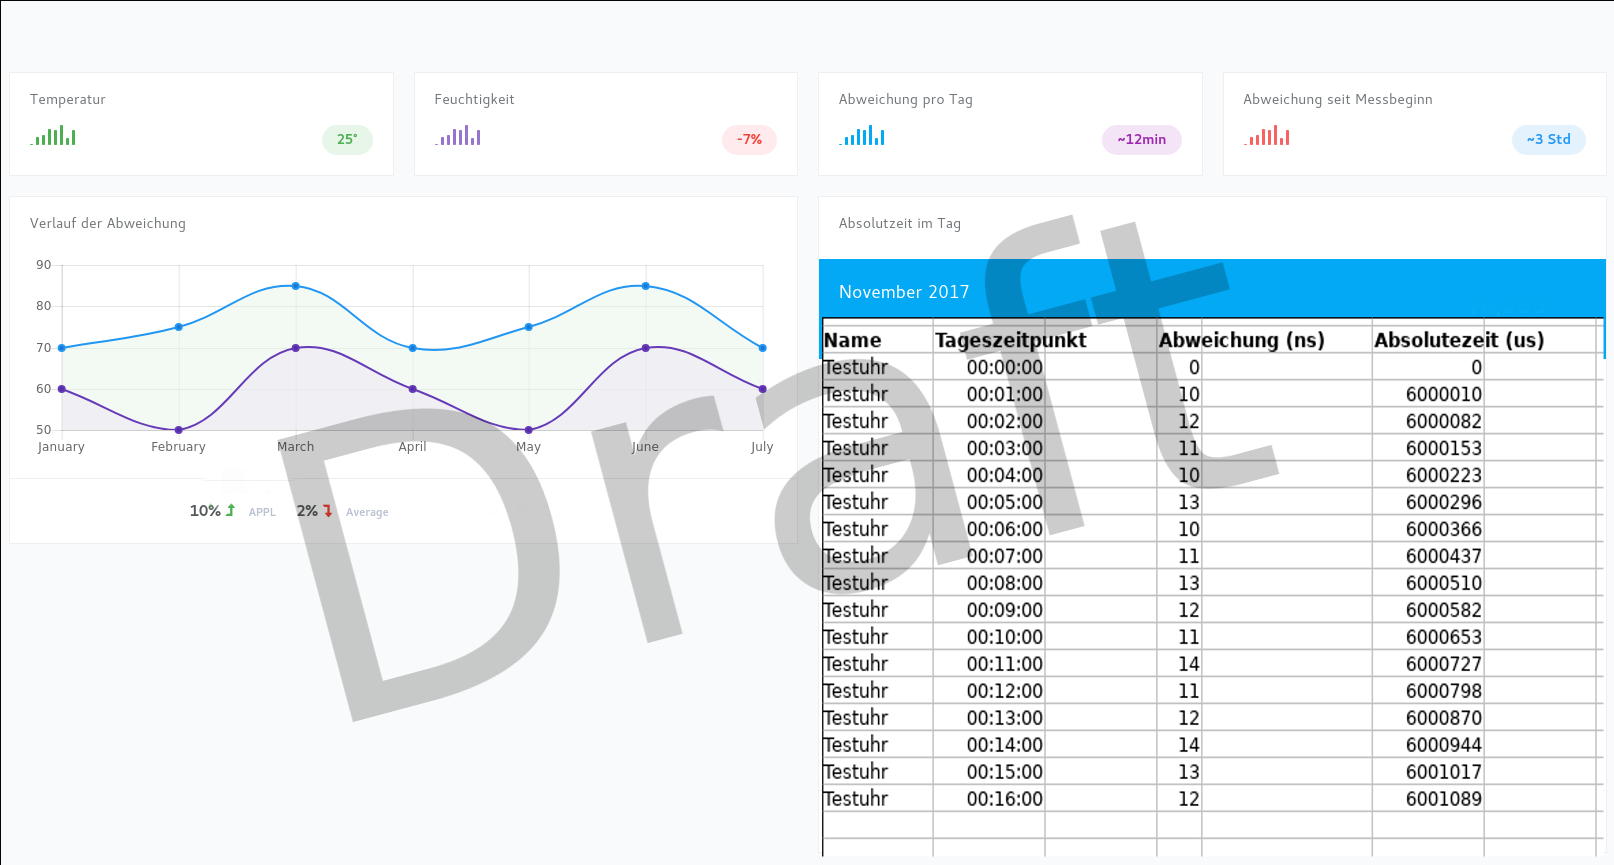
\includegraphics[width=\textwidth]{webclient_draft}
\end{figure}